
% Default to the notebook output style

    


% Inherit from the specified cell style.




    
\documentclass[11pt]{article}

    
    
    \usepackage[T1]{fontenc}
    % Nicer default font (+ math font) than Computer Modern for most use cases
    \usepackage{mathpazo}

    % Basic figure setup, for now with no caption control since it's done
    % automatically by Pandoc (which extracts ![](path) syntax from Markdown).
    \usepackage{graphicx}
    % We will generate all images so they have a width \maxwidth. This means
    % that they will get their normal width if they fit onto the page, but
    % are scaled down if they would overflow the margins.
    \makeatletter
    \def\maxwidth{\ifdim\Gin@nat@width>\linewidth\linewidth
    \else\Gin@nat@width\fi}
    \makeatother
    \let\Oldincludegraphics\includegraphics
    % Set max figure width to be 80% of text width, for now hardcoded.
    \renewcommand{\includegraphics}[1]{\Oldincludegraphics[width=.8\maxwidth]{#1}}
    % Ensure that by default, figures have no caption (until we provide a
    % proper Figure object with a Caption API and a way to capture that
    % in the conversion process - todo).
    \usepackage{caption}
    \DeclareCaptionLabelFormat{nolabel}{}
    \captionsetup{labelformat=nolabel}

    \usepackage{adjustbox} % Used to constrain images to a maximum size 
    \usepackage{xcolor} % Allow colors to be defined
    \usepackage{enumerate} % Needed for markdown enumerations to work
    \usepackage{geometry} % Used to adjust the document margins
    \usepackage{amsmath} % Equations
    \usepackage{amssymb} % Equations
    \usepackage{textcomp} % defines textquotesingle
    % Hack from http://tex.stackexchange.com/a/47451/13684:
    \AtBeginDocument{%
        \def\PYZsq{\textquotesingle}% Upright quotes in Pygmentized code
    }
    \usepackage{upquote} % Upright quotes for verbatim code
    \usepackage{eurosym} % defines \euro
    \usepackage[mathletters]{ucs} % Extended unicode (utf-8) support
    \usepackage[utf8x]{inputenc} % Allow utf-8 characters in the tex document
    \usepackage{fancyvrb} % verbatim replacement that allows latex
    \usepackage{grffile} % extends the file name processing of package graphics 
                         % to support a larger range 
    % The hyperref package gives us a pdf with properly built
    % internal navigation ('pdf bookmarks' for the table of contents,
    % internal cross-reference links, web links for URLs, etc.)
    \usepackage{hyperref}
    \usepackage{longtable} % longtable support required by pandoc >1.10
    \usepackage{booktabs}  % table support for pandoc > 1.12.2
    \usepackage[inline]{enumitem} % IRkernel/repr support (it uses the enumerate* environment)
    \usepackage[normalem]{ulem} % ulem is needed to support strikethroughs (\sout)
                                % normalem makes italics be italics, not underlines
    

    
    
    % Colors for the hyperref package
    \definecolor{urlcolor}{rgb}{0,.145,.698}
    \definecolor{linkcolor}{rgb}{.71,0.21,0.01}
    \definecolor{citecolor}{rgb}{.12,.54,.11}

    % ANSI colors
    \definecolor{ansi-black}{HTML}{3E424D}
    \definecolor{ansi-black-intense}{HTML}{282C36}
    \definecolor{ansi-red}{HTML}{E75C58}
    \definecolor{ansi-red-intense}{HTML}{B22B31}
    \definecolor{ansi-green}{HTML}{00A250}
    \definecolor{ansi-green-intense}{HTML}{007427}
    \definecolor{ansi-yellow}{HTML}{DDB62B}
    \definecolor{ansi-yellow-intense}{HTML}{B27D12}
    \definecolor{ansi-blue}{HTML}{208FFB}
    \definecolor{ansi-blue-intense}{HTML}{0065CA}
    \definecolor{ansi-magenta}{HTML}{D160C4}
    \definecolor{ansi-magenta-intense}{HTML}{A03196}
    \definecolor{ansi-cyan}{HTML}{60C6C8}
    \definecolor{ansi-cyan-intense}{HTML}{258F8F}
    \definecolor{ansi-white}{HTML}{C5C1B4}
    \definecolor{ansi-white-intense}{HTML}{A1A6B2}

    % commands and environments needed by pandoc snippets
    % extracted from the output of `pandoc -s`
    \providecommand{\tightlist}{%
      \setlength{\itemsep}{0pt}\setlength{\parskip}{0pt}}
    \DefineVerbatimEnvironment{Highlighting}{Verbatim}{commandchars=\\\{\}}
    % Add ',fontsize=\small' for more characters per line
    \newenvironment{Shaded}{}{}
    \newcommand{\KeywordTok}[1]{\textcolor[rgb]{0.00,0.44,0.13}{\textbf{{#1}}}}
    \newcommand{\DataTypeTok}[1]{\textcolor[rgb]{0.56,0.13,0.00}{{#1}}}
    \newcommand{\DecValTok}[1]{\textcolor[rgb]{0.25,0.63,0.44}{{#1}}}
    \newcommand{\BaseNTok}[1]{\textcolor[rgb]{0.25,0.63,0.44}{{#1}}}
    \newcommand{\FloatTok}[1]{\textcolor[rgb]{0.25,0.63,0.44}{{#1}}}
    \newcommand{\CharTok}[1]{\textcolor[rgb]{0.25,0.44,0.63}{{#1}}}
    \newcommand{\StringTok}[1]{\textcolor[rgb]{0.25,0.44,0.63}{{#1}}}
    \newcommand{\CommentTok}[1]{\textcolor[rgb]{0.38,0.63,0.69}{\textit{{#1}}}}
    \newcommand{\OtherTok}[1]{\textcolor[rgb]{0.00,0.44,0.13}{{#1}}}
    \newcommand{\AlertTok}[1]{\textcolor[rgb]{1.00,0.00,0.00}{\textbf{{#1}}}}
    \newcommand{\FunctionTok}[1]{\textcolor[rgb]{0.02,0.16,0.49}{{#1}}}
    \newcommand{\RegionMarkerTok}[1]{{#1}}
    \newcommand{\ErrorTok}[1]{\textcolor[rgb]{1.00,0.00,0.00}{\textbf{{#1}}}}
    \newcommand{\NormalTok}[1]{{#1}}
    
    % Additional commands for more recent versions of Pandoc
    \newcommand{\ConstantTok}[1]{\textcolor[rgb]{0.53,0.00,0.00}{{#1}}}
    \newcommand{\SpecialCharTok}[1]{\textcolor[rgb]{0.25,0.44,0.63}{{#1}}}
    \newcommand{\VerbatimStringTok}[1]{\textcolor[rgb]{0.25,0.44,0.63}{{#1}}}
    \newcommand{\SpecialStringTok}[1]{\textcolor[rgb]{0.73,0.40,0.53}{{#1}}}
    \newcommand{\ImportTok}[1]{{#1}}
    \newcommand{\DocumentationTok}[1]{\textcolor[rgb]{0.73,0.13,0.13}{\textit{{#1}}}}
    \newcommand{\AnnotationTok}[1]{\textcolor[rgb]{0.38,0.63,0.69}{\textbf{\textit{{#1}}}}}
    \newcommand{\CommentVarTok}[1]{\textcolor[rgb]{0.38,0.63,0.69}{\textbf{\textit{{#1}}}}}
    \newcommand{\VariableTok}[1]{\textcolor[rgb]{0.10,0.09,0.49}{{#1}}}
    \newcommand{\ControlFlowTok}[1]{\textcolor[rgb]{0.00,0.44,0.13}{\textbf{{#1}}}}
    \newcommand{\OperatorTok}[1]{\textcolor[rgb]{0.40,0.40,0.40}{{#1}}}
    \newcommand{\BuiltInTok}[1]{{#1}}
    \newcommand{\ExtensionTok}[1]{{#1}}
    \newcommand{\PreprocessorTok}[1]{\textcolor[rgb]{0.74,0.48,0.00}{{#1}}}
    \newcommand{\AttributeTok}[1]{\textcolor[rgb]{0.49,0.56,0.16}{{#1}}}
    \newcommand{\InformationTok}[1]{\textcolor[rgb]{0.38,0.63,0.69}{\textbf{\textit{{#1}}}}}
    \newcommand{\WarningTok}[1]{\textcolor[rgb]{0.38,0.63,0.69}{\textbf{\textit{{#1}}}}}
    
    
    % Define a nice break command that doesn't care if a line doesn't already
    % exist.
    \def\br{\hspace*{\fill} \\* }
    % Math Jax compatability definitions
    \def\gt{>}
    \def\lt{<}
    % Document parameters
    \title{Stayz\_Bookings\_Prediction}
    
    
    

    % Pygments definitions
    
\makeatletter
\def\PY@reset{\let\PY@it=\relax \let\PY@bf=\relax%
    \let\PY@ul=\relax \let\PY@tc=\relax%
    \let\PY@bc=\relax \let\PY@ff=\relax}
\def\PY@tok#1{\csname PY@tok@#1\endcsname}
\def\PY@toks#1+{\ifx\relax#1\empty\else%
    \PY@tok{#1}\expandafter\PY@toks\fi}
\def\PY@do#1{\PY@bc{\PY@tc{\PY@ul{%
    \PY@it{\PY@bf{\PY@ff{#1}}}}}}}
\def\PY#1#2{\PY@reset\PY@toks#1+\relax+\PY@do{#2}}

\expandafter\def\csname PY@tok@w\endcsname{\def\PY@tc##1{\textcolor[rgb]{0.73,0.73,0.73}{##1}}}
\expandafter\def\csname PY@tok@c\endcsname{\let\PY@it=\textit\def\PY@tc##1{\textcolor[rgb]{0.25,0.50,0.50}{##1}}}
\expandafter\def\csname PY@tok@cp\endcsname{\def\PY@tc##1{\textcolor[rgb]{0.74,0.48,0.00}{##1}}}
\expandafter\def\csname PY@tok@k\endcsname{\let\PY@bf=\textbf\def\PY@tc##1{\textcolor[rgb]{0.00,0.50,0.00}{##1}}}
\expandafter\def\csname PY@tok@kp\endcsname{\def\PY@tc##1{\textcolor[rgb]{0.00,0.50,0.00}{##1}}}
\expandafter\def\csname PY@tok@kt\endcsname{\def\PY@tc##1{\textcolor[rgb]{0.69,0.00,0.25}{##1}}}
\expandafter\def\csname PY@tok@o\endcsname{\def\PY@tc##1{\textcolor[rgb]{0.40,0.40,0.40}{##1}}}
\expandafter\def\csname PY@tok@ow\endcsname{\let\PY@bf=\textbf\def\PY@tc##1{\textcolor[rgb]{0.67,0.13,1.00}{##1}}}
\expandafter\def\csname PY@tok@nb\endcsname{\def\PY@tc##1{\textcolor[rgb]{0.00,0.50,0.00}{##1}}}
\expandafter\def\csname PY@tok@nf\endcsname{\def\PY@tc##1{\textcolor[rgb]{0.00,0.00,1.00}{##1}}}
\expandafter\def\csname PY@tok@nc\endcsname{\let\PY@bf=\textbf\def\PY@tc##1{\textcolor[rgb]{0.00,0.00,1.00}{##1}}}
\expandafter\def\csname PY@tok@nn\endcsname{\let\PY@bf=\textbf\def\PY@tc##1{\textcolor[rgb]{0.00,0.00,1.00}{##1}}}
\expandafter\def\csname PY@tok@ne\endcsname{\let\PY@bf=\textbf\def\PY@tc##1{\textcolor[rgb]{0.82,0.25,0.23}{##1}}}
\expandafter\def\csname PY@tok@nv\endcsname{\def\PY@tc##1{\textcolor[rgb]{0.10,0.09,0.49}{##1}}}
\expandafter\def\csname PY@tok@no\endcsname{\def\PY@tc##1{\textcolor[rgb]{0.53,0.00,0.00}{##1}}}
\expandafter\def\csname PY@tok@nl\endcsname{\def\PY@tc##1{\textcolor[rgb]{0.63,0.63,0.00}{##1}}}
\expandafter\def\csname PY@tok@ni\endcsname{\let\PY@bf=\textbf\def\PY@tc##1{\textcolor[rgb]{0.60,0.60,0.60}{##1}}}
\expandafter\def\csname PY@tok@na\endcsname{\def\PY@tc##1{\textcolor[rgb]{0.49,0.56,0.16}{##1}}}
\expandafter\def\csname PY@tok@nt\endcsname{\let\PY@bf=\textbf\def\PY@tc##1{\textcolor[rgb]{0.00,0.50,0.00}{##1}}}
\expandafter\def\csname PY@tok@nd\endcsname{\def\PY@tc##1{\textcolor[rgb]{0.67,0.13,1.00}{##1}}}
\expandafter\def\csname PY@tok@s\endcsname{\def\PY@tc##1{\textcolor[rgb]{0.73,0.13,0.13}{##1}}}
\expandafter\def\csname PY@tok@sd\endcsname{\let\PY@it=\textit\def\PY@tc##1{\textcolor[rgb]{0.73,0.13,0.13}{##1}}}
\expandafter\def\csname PY@tok@si\endcsname{\let\PY@bf=\textbf\def\PY@tc##1{\textcolor[rgb]{0.73,0.40,0.53}{##1}}}
\expandafter\def\csname PY@tok@se\endcsname{\let\PY@bf=\textbf\def\PY@tc##1{\textcolor[rgb]{0.73,0.40,0.13}{##1}}}
\expandafter\def\csname PY@tok@sr\endcsname{\def\PY@tc##1{\textcolor[rgb]{0.73,0.40,0.53}{##1}}}
\expandafter\def\csname PY@tok@ss\endcsname{\def\PY@tc##1{\textcolor[rgb]{0.10,0.09,0.49}{##1}}}
\expandafter\def\csname PY@tok@sx\endcsname{\def\PY@tc##1{\textcolor[rgb]{0.00,0.50,0.00}{##1}}}
\expandafter\def\csname PY@tok@m\endcsname{\def\PY@tc##1{\textcolor[rgb]{0.40,0.40,0.40}{##1}}}
\expandafter\def\csname PY@tok@gh\endcsname{\let\PY@bf=\textbf\def\PY@tc##1{\textcolor[rgb]{0.00,0.00,0.50}{##1}}}
\expandafter\def\csname PY@tok@gu\endcsname{\let\PY@bf=\textbf\def\PY@tc##1{\textcolor[rgb]{0.50,0.00,0.50}{##1}}}
\expandafter\def\csname PY@tok@gd\endcsname{\def\PY@tc##1{\textcolor[rgb]{0.63,0.00,0.00}{##1}}}
\expandafter\def\csname PY@tok@gi\endcsname{\def\PY@tc##1{\textcolor[rgb]{0.00,0.63,0.00}{##1}}}
\expandafter\def\csname PY@tok@gr\endcsname{\def\PY@tc##1{\textcolor[rgb]{1.00,0.00,0.00}{##1}}}
\expandafter\def\csname PY@tok@ge\endcsname{\let\PY@it=\textit}
\expandafter\def\csname PY@tok@gs\endcsname{\let\PY@bf=\textbf}
\expandafter\def\csname PY@tok@gp\endcsname{\let\PY@bf=\textbf\def\PY@tc##1{\textcolor[rgb]{0.00,0.00,0.50}{##1}}}
\expandafter\def\csname PY@tok@go\endcsname{\def\PY@tc##1{\textcolor[rgb]{0.53,0.53,0.53}{##1}}}
\expandafter\def\csname PY@tok@gt\endcsname{\def\PY@tc##1{\textcolor[rgb]{0.00,0.27,0.87}{##1}}}
\expandafter\def\csname PY@tok@err\endcsname{\def\PY@bc##1{\setlength{\fboxsep}{0pt}\fcolorbox[rgb]{1.00,0.00,0.00}{1,1,1}{\strut ##1}}}
\expandafter\def\csname PY@tok@kc\endcsname{\let\PY@bf=\textbf\def\PY@tc##1{\textcolor[rgb]{0.00,0.50,0.00}{##1}}}
\expandafter\def\csname PY@tok@kd\endcsname{\let\PY@bf=\textbf\def\PY@tc##1{\textcolor[rgb]{0.00,0.50,0.00}{##1}}}
\expandafter\def\csname PY@tok@kn\endcsname{\let\PY@bf=\textbf\def\PY@tc##1{\textcolor[rgb]{0.00,0.50,0.00}{##1}}}
\expandafter\def\csname PY@tok@kr\endcsname{\let\PY@bf=\textbf\def\PY@tc##1{\textcolor[rgb]{0.00,0.50,0.00}{##1}}}
\expandafter\def\csname PY@tok@bp\endcsname{\def\PY@tc##1{\textcolor[rgb]{0.00,0.50,0.00}{##1}}}
\expandafter\def\csname PY@tok@fm\endcsname{\def\PY@tc##1{\textcolor[rgb]{0.00,0.00,1.00}{##1}}}
\expandafter\def\csname PY@tok@vc\endcsname{\def\PY@tc##1{\textcolor[rgb]{0.10,0.09,0.49}{##1}}}
\expandafter\def\csname PY@tok@vg\endcsname{\def\PY@tc##1{\textcolor[rgb]{0.10,0.09,0.49}{##1}}}
\expandafter\def\csname PY@tok@vi\endcsname{\def\PY@tc##1{\textcolor[rgb]{0.10,0.09,0.49}{##1}}}
\expandafter\def\csname PY@tok@vm\endcsname{\def\PY@tc##1{\textcolor[rgb]{0.10,0.09,0.49}{##1}}}
\expandafter\def\csname PY@tok@sa\endcsname{\def\PY@tc##1{\textcolor[rgb]{0.73,0.13,0.13}{##1}}}
\expandafter\def\csname PY@tok@sb\endcsname{\def\PY@tc##1{\textcolor[rgb]{0.73,0.13,0.13}{##1}}}
\expandafter\def\csname PY@tok@sc\endcsname{\def\PY@tc##1{\textcolor[rgb]{0.73,0.13,0.13}{##1}}}
\expandafter\def\csname PY@tok@dl\endcsname{\def\PY@tc##1{\textcolor[rgb]{0.73,0.13,0.13}{##1}}}
\expandafter\def\csname PY@tok@s2\endcsname{\def\PY@tc##1{\textcolor[rgb]{0.73,0.13,0.13}{##1}}}
\expandafter\def\csname PY@tok@sh\endcsname{\def\PY@tc##1{\textcolor[rgb]{0.73,0.13,0.13}{##1}}}
\expandafter\def\csname PY@tok@s1\endcsname{\def\PY@tc##1{\textcolor[rgb]{0.73,0.13,0.13}{##1}}}
\expandafter\def\csname PY@tok@mb\endcsname{\def\PY@tc##1{\textcolor[rgb]{0.40,0.40,0.40}{##1}}}
\expandafter\def\csname PY@tok@mf\endcsname{\def\PY@tc##1{\textcolor[rgb]{0.40,0.40,0.40}{##1}}}
\expandafter\def\csname PY@tok@mh\endcsname{\def\PY@tc##1{\textcolor[rgb]{0.40,0.40,0.40}{##1}}}
\expandafter\def\csname PY@tok@mi\endcsname{\def\PY@tc##1{\textcolor[rgb]{0.40,0.40,0.40}{##1}}}
\expandafter\def\csname PY@tok@il\endcsname{\def\PY@tc##1{\textcolor[rgb]{0.40,0.40,0.40}{##1}}}
\expandafter\def\csname PY@tok@mo\endcsname{\def\PY@tc##1{\textcolor[rgb]{0.40,0.40,0.40}{##1}}}
\expandafter\def\csname PY@tok@ch\endcsname{\let\PY@it=\textit\def\PY@tc##1{\textcolor[rgb]{0.25,0.50,0.50}{##1}}}
\expandafter\def\csname PY@tok@cm\endcsname{\let\PY@it=\textit\def\PY@tc##1{\textcolor[rgb]{0.25,0.50,0.50}{##1}}}
\expandafter\def\csname PY@tok@cpf\endcsname{\let\PY@it=\textit\def\PY@tc##1{\textcolor[rgb]{0.25,0.50,0.50}{##1}}}
\expandafter\def\csname PY@tok@c1\endcsname{\let\PY@it=\textit\def\PY@tc##1{\textcolor[rgb]{0.25,0.50,0.50}{##1}}}
\expandafter\def\csname PY@tok@cs\endcsname{\let\PY@it=\textit\def\PY@tc##1{\textcolor[rgb]{0.25,0.50,0.50}{##1}}}

\def\PYZbs{\char`\\}
\def\PYZus{\char`\_}
\def\PYZob{\char`\{}
\def\PYZcb{\char`\}}
\def\PYZca{\char`\^}
\def\PYZam{\char`\&}
\def\PYZlt{\char`\<}
\def\PYZgt{\char`\>}
\def\PYZsh{\char`\#}
\def\PYZpc{\char`\%}
\def\PYZdl{\char`\$}
\def\PYZhy{\char`\-}
\def\PYZsq{\char`\'}
\def\PYZdq{\char`\"}
\def\PYZti{\char`\~}
% for compatibility with earlier versions
\def\PYZat{@}
\def\PYZlb{[}
\def\PYZrb{]}
\makeatother


    % Exact colors from NB
    \definecolor{incolor}{rgb}{0.0, 0.0, 0.5}
    \definecolor{outcolor}{rgb}{0.545, 0.0, 0.0}



    
    % Prevent overflowing lines due to hard-to-break entities
    \sloppy 
    % Setup hyperref package
    \hypersetup{
      breaklinks=true,  % so long urls are correctly broken across lines
      colorlinks=true,
      urlcolor=urlcolor,
      linkcolor=linkcolor,
      citecolor=citecolor,
      }
    % Slightly bigger margins than the latex defaults
    
    \geometry{verbose,tmargin=1in,bmargin=1in,lmargin=1in,rmargin=1in}
    
    

    \begin{document}
    
    
    \maketitle
    
    

    
    \section{Rental Accomodation Booking
Predictor}\label{rental-accomodation-booking-predictor}

For the last 3 months I have been running some web scraping jobs to
extract the publicly available data for short term holiday rentals in
NSW from an AirBnB type of website. Extracting the property details as
well as the public calendar allows us to get both the property features
as well as see the current state of bookings, specifically which dates
are currently booked and for how long.

The image below shows the location of all the properties, with Sydney
shown as the red dot:

\begin{figure}
\centering
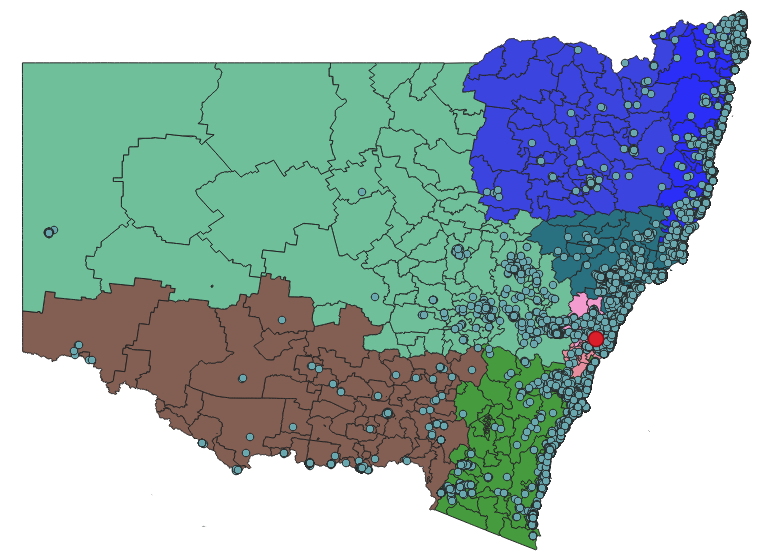
\includegraphics{Airbnb_Property_Locations_NSW.PNG}
\caption{Property Locations}
\end{figure}

Features that we are able to extract include: * Number of bedrooms *
Number of guests allowed * Price per night * Overall rating and the
number of reviews given * Distance and direction from Sydney * Number of
photos of the property on the listing * Word count of the main
description * The type of property (cottage, apartment, farmstay, house
etc) * Other features extracted from the listing begin with 'f\_' such
as \texttt{f\_clothes\_dryer} * Calendar showing current forward
bookings

The calendar information shows arrival and departure dates as part of
the html code, which can be parsed with Python and then collated to
provide the number of days booked. Future improvements will include
breaking this down into the number of weekends, public holidays, and
school holiday bookings.

\begin{figure}
\centering
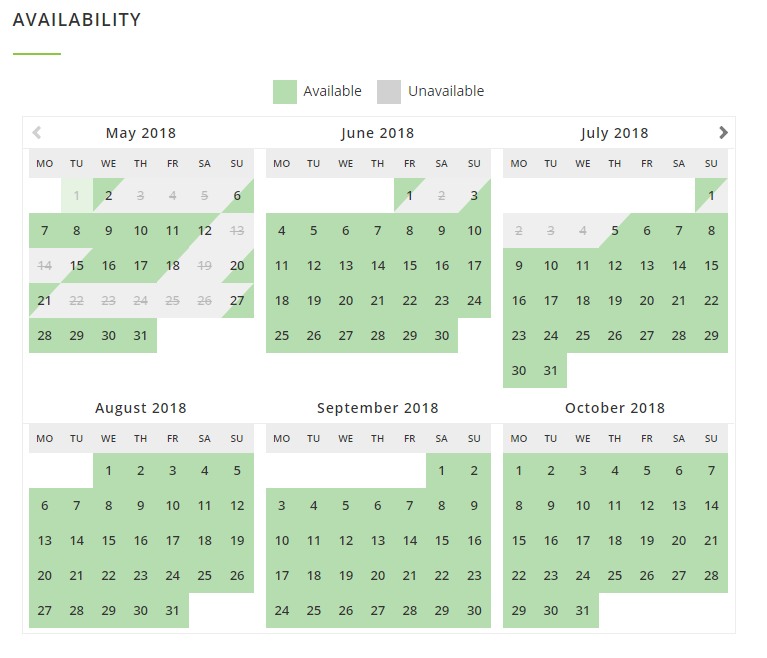
\includegraphics{Airbnb_Calendar.PNG}
\caption{Calendar}
\end{figure}

From manual inspection there are a small number of property listings who
get high bookings, with a large number of property listings having very
few or zero bookings.

The hypothesis is that there is an identifiable feature list which is
desirable for bookings, and therefore that bookings can be predicted
accurately for a new property when given the full set of features of
that property.

Based on the tutorial at
https://mitrai.com/tech-guide/using-aws-sagemaker-linear-regression-to-predict-store-transactions/

    \subsection{1. Import Libraries}\label{import-libraries}

    \begin{Verbatim}[commandchars=\\\{\}]
{\color{incolor}In [{\color{incolor} }]:} \PY{k+kn}{import} \PY{n+nn}{pandas} \PY{k}{as} \PY{n+nn}{pd}
        \PY{k+kn}{import} \PY{n+nn}{numpy} \PY{k}{as} \PY{n+nn}{np}
        \PY{k+kn}{import} \PY{n+nn}{matplotlib}\PY{n+nn}{.}\PY{n+nn}{pyplot} \PY{k}{as} \PY{n+nn}{plt}
        \PY{k+kn}{import} \PY{n+nn}{io}
        \PY{k+kn}{import} \PY{n+nn}{os}
        \PY{k+kn}{import} \PY{n+nn}{time}
        \PY{k+kn}{import} \PY{n+nn}{json}
        \PY{k+kn}{import} \PY{n+nn}{boto3}
        \PY{k+kn}{import} \PY{n+nn}{re}
        
        \PY{k+kn}{from} \PY{n+nn}{sklearn}\PY{n+nn}{.}\PY{n+nn}{model\PYZus{}selection} \PY{k}{import} \PY{n}{train\PYZus{}test\PYZus{}split}
        
        \PY{k+kn}{import} \PY{n+nn}{sagemaker}
        \PY{k+kn}{import} \PY{n+nn}{sagemaker}\PY{n+nn}{.}\PY{n+nn}{amazon}\PY{n+nn}{.}\PY{n+nn}{common} \PY{k}{as} \PY{n+nn}{smac}
        \PY{k+kn}{from} \PY{n+nn}{sagemaker}\PY{n+nn}{.}\PY{n+nn}{predictor} \PY{k}{import} \PY{n}{csv\PYZus{}serializer}\PY{p}{,} \PY{n}{json\PYZus{}deserializer}
        \PY{k+kn}{from} \PY{n+nn}{sagemaker} \PY{k}{import} \PY{n}{get\PYZus{}execution\PYZus{}role}
\end{Verbatim}


    \begin{Verbatim}[commandchars=\\\{\}]
{\color{incolor}In [{\color{incolor} }]:} \PY{n}{bucket} \PY{o}{=} \PY{l+s+s1}{\PYZsq{}}\PY{l+s+s1}{deloitte\PYZhy{}sagemaker}\PY{l+s+s1}{\PYZsq{}}
        \PY{n}{prefix} \PY{o}{=} \PY{l+s+s1}{\PYZsq{}}\PY{l+s+s1}{sagemaker/linear\PYZus{}time\PYZus{}series\PYZus{}forecast}\PY{l+s+s1}{\PYZsq{}}
        
        \PY{c+c1}{\PYZsh{} Define IAM role}
        \PY{c+c1}{\PYZsh{}role = get\PYZus{}execution\PYZus{}role()}
        \PY{c+c1}{\PYZsh{}role}
\end{Verbatim}


    \subsection{2. Data Import and
Validation}\label{data-import-and-validation}

    \begin{Verbatim}[commandchars=\\\{\}]
{\color{incolor}In [{\color{incolor} }]:} \PY{n}{hd\PYZus{}1} \PY{o}{=} \PY{n}{pd}\PY{o}{.}\PY{n}{read\PYZus{}csv}\PY{p}{(}\PY{l+s+s1}{\PYZsq{}}\PY{l+s+s1}{housing\PYZus{}sample.csv}\PY{l+s+s1}{\PYZsq{}}\PY{p}{)}
        
        \PY{c+c1}{\PYZsh{} Fill any \PYZsq{}NaN\PYZsq{} values with zero}
        \PY{n}{hd\PYZus{}1}\PY{o}{.}\PY{n}{fillna}\PY{p}{(}\PY{l+m+mi}{0}\PY{p}{,}\PY{n}{inplace}\PY{o}{=}\PY{k+kc}{True}\PY{p}{)}
        
        \PY{c+c1}{\PYZsh{} Drop the \PYZsq{}ext\PYZus{}at\PYZsq{} column}
        \PY{n}{hd\PYZus{}1}\PY{o}{.}\PY{n}{drop}\PY{p}{(}\PY{l+s+s1}{\PYZsq{}}\PY{l+s+s1}{ext\PYZus{}at}\PY{l+s+s1}{\PYZsq{}}\PY{p}{,}\PY{n}{axis}\PY{o}{=}\PY{l+m+mi}{1}\PY{p}{,} \PY{n}{inplace}\PY{o}{=}\PY{k+kc}{True}\PY{p}{)}
        
        \PY{c+c1}{\PYZsh{} Exclude any rows there the \PYZsq{}init\PYZus{}price\PYZsq{} is unknown.}
        \PY{n}{hd\PYZus{}2} \PY{o}{=} \PY{n}{hd\PYZus{}1}\PY{p}{[}\PY{n}{hd\PYZus{}1}\PY{p}{[}\PY{l+s+s1}{\PYZsq{}}\PY{l+s+s1}{init\PYZus{}price}\PY{l+s+s1}{\PYZsq{}}\PY{p}{]} \PY{o}{\PYZgt{}} \PY{l+m+mi}{0} \PY{p}{]}
        
        \PY{c+c1}{\PYZsh{} Drop the \PYZsq{}property\PYZus{}id\PYZsq{} column}
        \PY{n}{hd\PYZus{}3} \PY{o}{=} \PY{n}{hd\PYZus{}2}\PY{o}{.}\PY{n}{drop}\PY{p}{(}\PY{l+s+s1}{\PYZsq{}}\PY{l+s+s1}{property\PYZus{}id}\PY{l+s+s1}{\PYZsq{}}\PY{p}{,}\PY{n}{axis}\PY{o}{=}\PY{l+m+mi}{1}\PY{p}{)}
        
        \PY{n}{h\PYZus{}data} \PY{o}{=} \PY{n}{hd\PYZus{}3}
        
        
        \PY{n}{display}\PY{p}{(}\PY{n}{h\PYZus{}data}\PY{o}{.}\PY{n}{head}\PY{p}{(}\PY{p}{)}\PY{p}{)}
\end{Verbatim}


    \begin{Verbatim}[commandchars=\\\{\}]
{\color{incolor}In [{\color{incolor} }]:} \PY{c+c1}{\PYZsh{} Check for any missing postcodes}
        \PY{n}{mp} \PY{o}{=} \PY{n}{h\PYZus{}data}\PY{p}{[}\PY{n}{h\PYZus{}data}\PY{p}{[}\PY{l+s+s1}{\PYZsq{}}\PY{l+s+s1}{postcode}\PY{l+s+s1}{\PYZsq{}}\PY{p}{]}\PY{o}{.}\PY{n}{isnull}\PY{p}{(}\PY{p}{)}\PY{p}{]}
        \PY{n}{mp}\PY{o}{.}\PY{n}{postcode}
\end{Verbatim}


    \begin{Verbatim}[commandchars=\\\{\}]
{\color{incolor}In [{\color{incolor} }]:} \PY{c+c1}{\PYZsh{} Make sure that all fields are non null}
        \PY{n}{h\PYZus{}data}\PY{o}{.}\PY{n}{info}\PY{p}{(}\PY{p}{)}
\end{Verbatim}


    \subsection{3. Training and Test Data
Sets}\label{training-and-test-data-sets}

We will use the \texttt{total\_booked\_days} column as being the y-value
we want to predict, then create training and test data sets using an
80/20 split.

    \begin{Verbatim}[commandchars=\\\{\}]
{\color{incolor}In [{\color{incolor} }]:} \PY{c+c1}{\PYZsh{} Define which column is the y variable}
        \PY{n}{y} \PY{o}{=} \PY{n}{h\PYZus{}data}\PY{o}{.}\PY{n}{total\PYZus{}booked\PYZus{}days}
        
        \PY{c+c1}{\PYZsh{} Split into a training set and a testing set}
        \PY{n}{X\PYZus{}train}\PY{p}{,} \PY{n}{X\PYZus{}test}\PY{p}{,} \PY{n}{y\PYZus{}train}\PY{p}{,} \PY{n}{y\PYZus{}test} \PY{o}{=} \PY{n}{train\PYZus{}test\PYZus{}split}\PY{p}{(}\PY{n}{h\PYZus{}data}\PY{p}{,} \PY{n}{y}\PY{p}{,} \PY{n}{test\PYZus{}size}\PY{o}{=}\PY{l+m+mf}{0.20}\PY{p}{,} \PY{n}{random\PYZus{}state}\PY{o}{=}\PY{l+m+mi}{42}\PY{p}{)}
        
        \PY{n}{X\PYZus{}train}\PY{o}{.}\PY{n}{head}\PY{p}{(}\PY{p}{)}
\end{Verbatim}


    \subsection{4. Convert Data and Upload to
S3}\label{convert-data-and-upload-to-s3}

    \begin{Verbatim}[commandchars=\\\{\}]
{\color{incolor}In [{\color{incolor} }]:} \PY{c+c1}{\PYZsh{} Convert training dataset to RecordIO format as required by Amazon Sagemaker}
        
        \PY{n}{buf} \PY{o}{=} \PY{n}{io}\PY{o}{.}\PY{n}{BytesIO}\PY{p}{(}\PY{p}{)}
        \PY{n}{smac}\PY{o}{.}\PY{n}{write\PYZus{}numpy\PYZus{}to\PYZus{}dense\PYZus{}tensor}\PY{p}{(}\PY{n}{buf}\PY{p}{,} \PY{n}{np}\PY{o}{.}\PY{n}{array}\PY{p}{(}\PY{n}{X\PYZus{}train}\PY{p}{)}\PY{o}{.}\PY{n}{astype}\PY{p}{(}\PY{l+s+s1}{\PYZsq{}}\PY{l+s+s1}{float32}\PY{l+s+s1}{\PYZsq{}}\PY{p}{)}\PY{p}{,} \PY{n}{np}\PY{o}{.}\PY{n}{array}\PY{p}{(}\PY{n}{y\PYZus{}train}\PY{p}{)}\PY{o}{.}\PY{n}{astype}\PY{p}{(}\PY{l+s+s1}{\PYZsq{}}\PY{l+s+s1}{float32}\PY{l+s+s1}{\PYZsq{}}\PY{p}{)}\PY{p}{)}
        \PY{n}{buf}\PY{o}{.}\PY{n}{seek}\PY{p}{(}\PY{l+m+mi}{0}\PY{p}{)}
\end{Verbatim}


    \begin{Verbatim}[commandchars=\\\{\}]
{\color{incolor}In [{\color{incolor} }]:} \PY{c+c1}{\PYZsh{} Upload training data to S3}
        
        \PY{n}{key} \PY{o}{=} \PY{l+s+s1}{\PYZsq{}}\PY{l+s+s1}{housing\PYZus{}data.data}\PY{l+s+s1}{\PYZsq{}}
        \PY{n}{boto3}\PY{o}{.}\PY{n}{resource}\PY{p}{(}\PY{l+s+s1}{\PYZsq{}}\PY{l+s+s1}{s3}\PY{l+s+s1}{\PYZsq{}}\PY{p}{)}\PY{o}{.}\PY{n}{Bucket}\PY{p}{(}\PY{n}{bucket}\PY{p}{)}\PY{o}{.}\PY{n}{Object}\PY{p}{(}\PY{n}{os}\PY{o}{.}\PY{n}{path}\PY{o}{.}\PY{n}{join}\PY{p}{(}\PY{n}{prefix}\PY{p}{,} \PY{l+s+s1}{\PYZsq{}}\PY{l+s+s1}{train}\PY{l+s+s1}{\PYZsq{}}\PY{p}{,} \PY{n}{key}\PY{p}{)}\PY{p}{)}\PY{o}{.}\PY{n}{upload\PYZus{}fileobj}\PY{p}{(}\PY{n}{buf}\PY{p}{)}
        \PY{n}{s3\PYZus{}train\PYZus{}data} \PY{o}{=} \PY{l+s+s1}{\PYZsq{}}\PY{l+s+s1}{s3://}\PY{l+s+si}{\PYZob{}\PYZcb{}}\PY{l+s+s1}{/}\PY{l+s+si}{\PYZob{}\PYZcb{}}\PY{l+s+s1}{/train/}\PY{l+s+si}{\PYZob{}\PYZcb{}}\PY{l+s+s1}{\PYZsq{}}\PY{o}{.}\PY{n}{format}\PY{p}{(}\PY{n}{bucket}\PY{p}{,} \PY{n}{prefix}\PY{p}{,} \PY{n}{key}\PY{p}{)}
        \PY{n+nb}{print}\PY{p}{(}\PY{l+s+s1}{\PYZsq{}}\PY{l+s+s1}{Uploaded training data location: }\PY{l+s+si}{\PYZob{}\PYZcb{}}\PY{l+s+s1}{\PYZsq{}}\PY{o}{.}\PY{n}{format}\PY{p}{(}\PY{n}{s3\PYZus{}train\PYZus{}data}\PY{p}{)}\PY{p}{)}
\end{Verbatim}


    \begin{Verbatim}[commandchars=\\\{\}]
{\color{incolor}In [{\color{incolor} }]:} \PY{c+c1}{\PYZsh{} Convert validation dataset to RecordIO format as required by Amazon Sagemaker}
        
        \PY{n}{buf} \PY{o}{=} \PY{n}{io}\PY{o}{.}\PY{n}{BytesIO}\PY{p}{(}\PY{p}{)}
        \PY{n}{smac}\PY{o}{.}\PY{n}{write\PYZus{}numpy\PYZus{}to\PYZus{}dense\PYZus{}tensor}\PY{p}{(}\PY{n}{buf}\PY{p}{,} \PY{n}{np}\PY{o}{.}\PY{n}{array}\PY{p}{(}\PY{n}{X\PYZus{}test}\PY{p}{)}\PY{o}{.}\PY{n}{astype}\PY{p}{(}\PY{l+s+s1}{\PYZsq{}}\PY{l+s+s1}{float32}\PY{l+s+s1}{\PYZsq{}}\PY{p}{)}\PY{p}{,} \PY{n}{np}\PY{o}{.}\PY{n}{array}\PY{p}{(}\PY{n}{y\PYZus{}test}\PY{p}{)}\PY{o}{.}\PY{n}{astype}\PY{p}{(}\PY{l+s+s1}{\PYZsq{}}\PY{l+s+s1}{float32}\PY{l+s+s1}{\PYZsq{}}\PY{p}{)}\PY{p}{)}
        \PY{n}{buf}\PY{o}{.}\PY{n}{seek}\PY{p}{(}\PY{l+m+mi}{0}\PY{p}{)}
\end{Verbatim}


    \begin{Verbatim}[commandchars=\\\{\}]
{\color{incolor}In [{\color{incolor} }]:} \PY{c+c1}{\PYZsh{} Upload validation data to S3}
        
        \PY{n}{key} \PY{o}{=} \PY{l+s+s1}{\PYZsq{}}\PY{l+s+s1}{housing\PYZus{}validation.data}\PY{l+s+s1}{\PYZsq{}}
        \PY{n}{boto3}\PY{o}{.}\PY{n}{resource}\PY{p}{(}\PY{l+s+s1}{\PYZsq{}}\PY{l+s+s1}{s3}\PY{l+s+s1}{\PYZsq{}}\PY{p}{)}\PY{o}{.}\PY{n}{Bucket}\PY{p}{(}\PY{n}{bucket}\PY{p}{)}\PY{o}{.}\PY{n}{Object}\PY{p}{(}\PY{n}{os}\PY{o}{.}\PY{n}{path}\PY{o}{.}\PY{n}{join}\PY{p}{(}\PY{n}{prefix}\PY{p}{,} \PY{l+s+s1}{\PYZsq{}}\PY{l+s+s1}{validation}\PY{l+s+s1}{\PYZsq{}}\PY{p}{,} \PY{n}{key}\PY{p}{)}\PY{p}{)}\PY{o}{.}\PY{n}{upload\PYZus{}fileobj}\PY{p}{(}\PY{n}{buf}\PY{p}{)}
        \PY{n}{s3\PYZus{}validation\PYZus{}data} \PY{o}{=} \PY{l+s+s1}{\PYZsq{}}\PY{l+s+s1}{s3://}\PY{l+s+si}{\PYZob{}\PYZcb{}}\PY{l+s+s1}{/}\PY{l+s+si}{\PYZob{}\PYZcb{}}\PY{l+s+s1}{/validation/}\PY{l+s+si}{\PYZob{}\PYZcb{}}\PY{l+s+s1}{\PYZsq{}}\PY{o}{.}\PY{n}{format}\PY{p}{(}\PY{n}{bucket}\PY{p}{,} \PY{n}{prefix}\PY{p}{,} \PY{n}{key}\PY{p}{)}
        \PY{n+nb}{print}\PY{p}{(}\PY{l+s+s1}{\PYZsq{}}\PY{l+s+s1}{Uploaded validation data location: }\PY{l+s+si}{\PYZob{}\PYZcb{}}\PY{l+s+s1}{\PYZsq{}}\PY{o}{.}\PY{n}{format}\PY{p}{(}\PY{n}{s3\PYZus{}validation\PYZus{}data}\PY{p}{)}\PY{p}{)}
\end{Verbatim}


    \subsubsection{5. Run LinearLearner
Predictor}\label{run-linearlearner-predictor}

    \begin{Verbatim}[commandchars=\\\{\}]
{\color{incolor}In [{\color{incolor} }]:} \PY{c+c1}{\PYZsh{} Specify the containers}
        
        \PY{n}{containers} \PY{o}{=} \PY{p}{\PYZob{}}\PY{l+s+s1}{\PYZsq{}}\PY{l+s+s1}{us\PYZhy{}west\PYZhy{}2}\PY{l+s+s1}{\PYZsq{}}\PY{p}{:} \PY{l+s+s1}{\PYZsq{}}\PY{l+s+s1}{174872318107.dkr.ecr.us\PYZhy{}west\PYZhy{}2.amazonaws.com/linear\PYZhy{}learner:latest}\PY{l+s+s1}{\PYZsq{}}\PY{p}{,}
                     \PY{l+s+s1}{\PYZsq{}}\PY{l+s+s1}{us\PYZhy{}east\PYZhy{}1}\PY{l+s+s1}{\PYZsq{}}\PY{p}{:} \PY{l+s+s1}{\PYZsq{}}\PY{l+s+s1}{382416733822.dkr.ecr.us\PYZhy{}east\PYZhy{}1.amazonaws.com/linear\PYZhy{}learner:latest}\PY{l+s+s1}{\PYZsq{}}\PY{p}{,}
                     \PY{l+s+s1}{\PYZsq{}}\PY{l+s+s1}{us\PYZhy{}east\PYZhy{}2}\PY{l+s+s1}{\PYZsq{}}\PY{p}{:} \PY{l+s+s1}{\PYZsq{}}\PY{l+s+s1}{404615174143.dkr.ecr.us\PYZhy{}east\PYZhy{}2.amazonaws.com/linear\PYZhy{}learner:latest}\PY{l+s+s1}{\PYZsq{}}\PY{p}{,}
                     \PY{l+s+s1}{\PYZsq{}}\PY{l+s+s1}{eu\PYZhy{}west\PYZhy{}1}\PY{l+s+s1}{\PYZsq{}}\PY{p}{:} \PY{l+s+s1}{\PYZsq{}}\PY{l+s+s1}{438346466558.dkr.ecr.eu\PYZhy{}west\PYZhy{}1.amazonaws.com/linear\PYZhy{}learner:latest}\PY{l+s+s1}{\PYZsq{}}\PY{p}{\PYZcb{}}
\end{Verbatim}


    \begin{Verbatim}[commandchars=\\\{\}]
{\color{incolor}In [{\color{incolor} }]:} \PY{c+c1}{\PYZsh{} Start a Sagemaker session}
        
        \PY{n}{sess} \PY{o}{=} \PY{n}{sagemaker}\PY{o}{.}\PY{n}{Session}\PY{p}{(}\PY{p}{)}
        
        \PY{n}{linear} \PY{o}{=} \PY{n}{sagemaker}\PY{o}{.}\PY{n}{estimator}\PY{o}{.}\PY{n}{Estimator}\PY{p}{(}\PY{n}{containers}\PY{p}{[}\PY{n}{boto3}\PY{o}{.}\PY{n}{Session}\PY{p}{(}\PY{p}{)}\PY{o}{.}\PY{n}{region\PYZus{}name}\PY{p}{]}
                                               \PY{p}{,}\PY{n}{role}
                                               \PY{p}{,}\PY{n}{train\PYZus{}instance\PYZus{}count}\PY{o}{=}\PY{l+m+mi}{1}
                                               \PY{p}{,}\PY{n}{train\PYZus{}instance\PYZus{}type}\PY{o}{=}\PY{l+s+s1}{\PYZsq{}}\PY{l+s+s1}{ml.m5.large}\PY{l+s+s1}{\PYZsq{}}
                                               \PY{p}{,}\PY{n}{output\PYZus{}path}\PY{o}{=}\PY{l+s+s1}{\PYZsq{}}\PY{l+s+s1}{s3://}\PY{l+s+si}{\PYZob{}\PYZcb{}}\PY{l+s+s1}{/}\PY{l+s+si}{\PYZob{}\PYZcb{}}\PY{l+s+s1}{/output}\PY{l+s+s1}{\PYZsq{}}\PY{o}{.}\PY{n}{format}\PY{p}{(}\PY{n}{bucket}\PY{p}{,} \PY{n}{prefix}\PY{p}{)}
                                               \PY{p}{,}\PY{n}{sagemaker\PYZus{}session}\PY{o}{=}\PY{n}{sess}\PY{p}{)}
        
        \PY{n}{linear}\PY{o}{.}\PY{n}{set\PYZus{}hyperparameters}\PY{p}{(}\PY{n}{feature\PYZus{}dim}\PY{o}{=}\PY{l+m+mi}{77}
                                   \PY{p}{,}\PY{n}{mini\PYZus{}batch\PYZus{}size}\PY{o}{=}\PY{l+m+mi}{100}
                                   \PY{p}{,}\PY{n}{predictor\PYZus{}type}\PY{o}{=}\PY{l+s+s1}{\PYZsq{}}\PY{l+s+s1}{regressor}\PY{l+s+s1}{\PYZsq{}}
                                   \PY{p}{,}\PY{n}{epochs}\PY{o}{=}\PY{l+m+mi}{10}
                                   \PY{p}{,}\PY{n}{num\PYZus{}models}\PY{o}{=}\PY{l+m+mi}{32}
                                   \PY{p}{,}\PY{n}{loss}\PY{o}{=}\PY{l+s+s1}{\PYZsq{}}\PY{l+s+s1}{absolute\PYZus{}loss}\PY{l+s+s1}{\PYZsq{}}\PY{p}{)}
        
        \PY{n}{linear}\PY{o}{.}\PY{n}{fit}\PY{p}{(}\PY{p}{\PYZob{}}\PY{l+s+s1}{\PYZsq{}}\PY{l+s+s1}{train}\PY{l+s+s1}{\PYZsq{}}\PY{p}{:} \PY{n}{s3\PYZus{}train\PYZus{}data}\PY{p}{,} \PY{l+s+s1}{\PYZsq{}}\PY{l+s+s1}{validation}\PY{l+s+s1}{\PYZsq{}}\PY{p}{:} \PY{n}{s3\PYZus{}validation\PYZus{}data}\PY{p}{\PYZcb{}}\PY{p}{)}
\end{Verbatim}


    \begin{Verbatim}[commandchars=\\\{\}]
{\color{incolor}In [{\color{incolor} }]:} \PY{n}{linear\PYZus{}predictor} \PY{o}{=} \PY{n}{linear}\PY{o}{.}\PY{n}{deploy}\PY{p}{(}\PY{n}{initial\PYZus{}instance\PYZus{}count}\PY{o}{=}\PY{l+m+mi}{1}\PY{p}{,}\PY{n}{instance\PYZus{}type}\PY{o}{=}\PY{l+s+s1}{\PYZsq{}}\PY{l+s+s1}{ml.m4.xlarge}\PY{l+s+s1}{\PYZsq{}}\PY{p}{)}
\end{Verbatim}


    Create a function to convert our numpy arrays into a format that can be
handled by the HTTP POST request we pass to the inference container. In
this case it's a simple CSV string. The results will be published back
as JSON. For these common formats we can use the Amazon SageMaker Python
SDK's built in csv\_serializer and json\_deserializer functions.

    \begin{Verbatim}[commandchars=\\\{\}]
{\color{incolor}In [{\color{incolor} }]:} \PY{n}{linear\PYZus{}predictor}\PY{o}{.}\PY{n}{content\PYZus{}type} \PY{o}{=} \PY{l+s+s1}{\PYZsq{}}\PY{l+s+s1}{text/csv}\PY{l+s+s1}{\PYZsq{}}
        \PY{n}{linear\PYZus{}predictor}\PY{o}{.}\PY{n}{serializer} \PY{o}{=} \PY{n}{csv\PYZus{}serializer}
        \PY{n}{linear\PYZus{}predictor}\PY{o}{.}\PY{n}{deserializer} \PY{o}{=} \PY{n}{json\PYZus{}deserializer}
\end{Verbatim}


    \subsection{7. Run Model with Test
Dataset}\label{run-model-with-test-dataset}

Now that the model has been deployed to an endpoint we can call this
model with the test dataset, then extract the predictions into the
\texttt{one\_step} variable

    \begin{Verbatim}[commandchars=\\\{\}]
{\color{incolor}In [{\color{incolor} }]:} \PY{n}{test\PYZus{}X} \PY{o}{=} \PY{n}{X\PYZus{}test}\PY{o}{.}\PY{n}{as\PYZus{}matrix}\PY{p}{(}\PY{p}{)}
        
        \PY{n}{result} \PY{o}{=} \PY{n}{linear\PYZus{}predictor}\PY{o}{.}\PY{n}{predict}\PY{p}{(}\PY{n}{test\PYZus{}X}\PY{p}{)}
        
        \PY{n}{one\PYZus{}step} \PY{o}{=} \PY{n}{np}\PY{o}{.}\PY{n}{array}\PY{p}{(}\PY{p}{[}\PY{n}{r}\PY{p}{[}\PY{l+s+s1}{\PYZsq{}}\PY{l+s+s1}{score}\PY{l+s+s1}{\PYZsq{}}\PY{p}{]} \PY{k}{for} \PY{n}{r} \PY{o+ow}{in} \PY{n}{result}\PY{p}{[}\PY{l+s+s1}{\PYZsq{}}\PY{l+s+s1}{predictions}\PY{l+s+s1}{\PYZsq{}}\PY{p}{]}\PY{p}{]}\PY{p}{)}
\end{Verbatim}


    \begin{Verbatim}[commandchars=\\\{\}]
{\color{incolor}In [{\color{incolor} }]:} \PY{c+c1}{\PYZsh{} Find some values from the test data to validate where the number of booked days is non zero}
        
        \PY{n}{X\PYZus{}test}\PY{p}{[}\PY{l+s+s1}{\PYZsq{}}\PY{l+s+s1}{total\PYZus{}booked\PYZus{}days}\PY{l+s+s1}{\PYZsq{}}\PY{p}{]}\PY{p}{[}\PY{l+m+mi}{0}\PY{p}{:}\PY{l+m+mi}{10}\PY{p}{]}
\end{Verbatim}


    \begin{Verbatim}[commandchars=\\\{\}]
{\color{incolor}In [{\color{incolor} }]:} \PY{c+c1}{\PYZsh{} Since the first item (index position 0) has some bookings we can look at the result vs the predicted result}
        \PY{n}{test\PYZus{}index} \PY{o}{=} \PY{l+m+mi}{0}
        
        \PY{n}{pred\PYZus{}price} \PY{o}{=} \PY{n}{one\PYZus{}step}\PY{p}{[}\PY{n}{test\PYZus{}index}\PY{p}{]}
        \PY{n+nb}{print}\PY{p}{(}\PY{l+s+s2}{\PYZdq{}}\PY{l+s+s2}{Prediction: }\PY{l+s+s2}{\PYZdq{}} \PY{o}{+} \PY{n+nb}{str}\PY{p}{(}\PY{n}{pred\PYZus{}price}\PY{p}{)}\PY{p}{)}
        
        \PY{n}{act\PYZus{}price} \PY{o}{=} \PY{n}{X\PYZus{}test}\PY{o}{.}\PY{n}{iloc}\PY{p}{[}\PY{n}{test\PYZus{}index}\PY{p}{]}\PY{p}{[}\PY{l+s+s1}{\PYZsq{}}\PY{l+s+s1}{total\PYZus{}booked\PYZus{}days}\PY{l+s+s1}{\PYZsq{}}\PY{p}{]}
        \PY{n+nb}{print}\PY{p}{(}\PY{l+s+s2}{\PYZdq{}}\PY{l+s+s2}{Actual: }\PY{l+s+s2}{\PYZdq{}} \PY{o}{+} \PY{n+nb}{str}\PY{p}{(}\PY{n}{act\PYZus{}price}\PY{p}{)}\PY{p}{)}
        
        \PY{n+nb}{print}\PY{p}{(}\PY{l+s+s2}{\PYZdq{}}\PY{l+s+s2}{Difference: }\PY{l+s+si}{\PYZob{}0:.2f\PYZcb{}}\PY{l+s+s2}{\PYZpc{}}\PY{l+s+s2}{\PYZdq{}}\PY{o}{.}\PY{n}{format}\PY{p}{(}\PY{p}{(}\PY{p}{(}\PY{p}{(}\PY{n}{act\PYZus{}price} \PY{o}{\PYZhy{}} \PY{n}{pred\PYZus{}price}\PY{p}{)}\PY{o}{/}\PY{n}{act\PYZus{}price}\PY{p}{)}\PY{o}{*}\PY{l+m+mi}{100}\PY{p}{)}\PY{p}{)}\PY{p}{)}
\end{Verbatim}


    Work out the difference between the prediction and the results for all
the test set

    \begin{Verbatim}[commandchars=\\\{\}]
{\color{incolor}In [{\color{incolor} }]:} \PY{k+kn}{from} \PY{n+nn}{numpy} \PY{k}{import} \PY{n}{inf}
        
        \PY{n}{res1} \PY{o}{=} \PY{p}{(}\PY{n}{np}\PY{o}{.}\PY{n}{abs}\PY{p}{(}\PY{n}{y\PYZus{}test} \PY{o}{\PYZhy{}} \PY{n}{one\PYZus{}step}\PY{p}{)} \PY{o}{/} \PY{n}{y\PYZus{}test}\PY{p}{)}
        
        \PY{c+c1}{\PYZsh{} If the result is \PYZsq{}inf\PYZsq{} then default to zero}
        \PY{n}{res1}\PY{p}{[}\PY{n}{res1} \PY{o}{==} \PY{n}{inf}\PY{p}{]} \PY{o}{=} \PY{l+m+mi}{0}
        
        \PY{n+nb}{print}\PY{p}{(}\PY{l+s+s2}{\PYZdq{}}\PY{l+s+s2}{Median differencet: }\PY{l+s+s2}{\PYZdq{}} \PY{o}{+} \PY{n+nb}{str}\PY{p}{(}\PY{n}{np}\PY{o}{.}\PY{n}{median}\PY{p}{(}\PY{n}{res1}\PY{p}{)}\PY{p}{)}\PY{p}{)}
        
        \PY{c+c1}{\PYZsh{} Check the first few records}
        \PY{n}{res1}\PY{p}{[}\PY{l+m+mi}{0}\PY{p}{:}\PY{l+m+mi}{5}\PY{p}{]}
\end{Verbatim}


    \subsection{8. Graph Results}\label{graph-results}

Graph the actual values vs predicted values for a slice of the dataset.

\textbf{Note:} The predicted values are all within a fraction of the
actual result, ie 17.0 vs 16.818 for the first element. This means that
the results are hard to see visually.

    \begin{Verbatim}[commandchars=\\\{\}]
{\color{incolor}In [{\color{incolor} }]:} \PY{n+nb}{print}\PY{p}{(}\PY{l+s+s1}{\PYZsq{}}\PY{l+s+s1}{One\PYZhy{}step = }\PY{l+s+s1}{\PYZsq{}}\PY{p}{,} \PY{n}{np}\PY{o}{.}\PY{n}{median}\PY{p}{(}\PY{n}{res1}\PY{p}{)}\PY{p}{)}
        
        \PY{n}{plt}\PY{o}{.}\PY{n}{figure}\PY{p}{(}\PY{n}{figsize}\PY{o}{=}\PY{p}{(}\PY{l+m+mi}{20}\PY{p}{,}\PY{l+m+mi}{10}\PY{p}{)}\PY{p}{)}
        
        \PY{n}{plt}\PY{o}{.}\PY{n}{plot}\PY{p}{(}\PY{n}{one\PYZus{}step}\PY{p}{[}\PY{l+m+mi}{200}\PY{p}{:}\PY{l+m+mi}{250}\PY{p}{]}\PY{p}{,} \PY{n}{label}\PY{o}{=}\PY{l+s+s1}{\PYZsq{}}\PY{l+s+s1}{forecast}\PY{l+s+s1}{\PYZsq{}}\PY{p}{)}
        \PY{n}{plt}\PY{o}{.}\PY{n}{plot}\PY{p}{(}\PY{n}{np}\PY{o}{.}\PY{n}{array}\PY{p}{(}\PY{n}{y\PYZus{}test}\PY{p}{[}\PY{l+m+mi}{200}\PY{p}{:}\PY{l+m+mi}{250}\PY{p}{]}\PY{p}{)}\PY{p}{,} \PY{n}{label}\PY{o}{=}\PY{l+s+s1}{\PYZsq{}}\PY{l+s+s1}{actual}\PY{l+s+s1}{\PYZsq{}}\PY{p}{)}
        \PY{n}{plt}\PY{o}{.}\PY{n}{legend}\PY{p}{(}\PY{p}{)}
        \PY{n}{plt}\PY{o}{.}\PY{n}{show}\PY{p}{(}\PY{p}{)}
\end{Verbatim}


    \begin{Verbatim}[commandchars=\\\{\}]
{\color{incolor}In [{\color{incolor} }]:} \PY{c+c1}{\PYZsh{} Run some housing details manually to see what changes}
        
        \PY{c+c1}{\PYZsh{}linear\PYZus{}predictor.predict() \PYZsh{}expected label to be 1}
\end{Verbatim}


    \subsubsection{(Optional) Clean-up}\label{optional-clean-up}

If you're ready to be done with this notebook, please run the cell
below. This will remove the hosted endpoint you created and avoid any
charges from a stray instance being left on.

    \begin{Verbatim}[commandchars=\\\{\}]
{\color{incolor}In [{\color{incolor} }]:} \PY{c+c1}{\PYZsh{}sess.delete\PYZus{}endpoint(linear\PYZus{}predictor.endpoint)}
\end{Verbatim}



    % Add a bibliography block to the postdoc
    
    
    
    \end{document}
